






































\section{Implementation}

\subsection{Preprocessor}

As described in section [xxx] preprocessing is done to create necessary files for rogue AP and malicious user detection. Additionally it is used to create {\em relevant files} which are needed by the neural network to learn correctly.

As shown in figure [xxx] the entry point for the WIDS is the {\em DataPreprocessor} class. When calling its {\em preprocess()} method the preprocessing starts by using the {\em RogueApManager}, {\em ClientMacManager}, {\em RelevantDataCreator} and the {\em ScaleManager} class.

The {\em preprocess()} method iterates through all packets in the normal traffic file and gives them to every class.

{\em {\bf RogueApManager}}

The RogueApManager is responsible to create a file named {\em ap.txt} which holds all APs found. First, it retrieves the BSSID of every single packet and then checks whether it is already available in the file. In case it is already listed then no new entry is made. In case it is not available yet the new BSSID is stored in the file.

{\em {\bf ClientMacManager}}

The ClientMacManager performs the same actions as the RogueApManager except that it does not read out the BSSID but the MAC address of the client and stores it in the {\em mac.txt} file.

\subsection{Feature Extraction}

\subsection{Neural Network}

Figure \ref{uml_wids} shows an UML diagram of the neural network displaying the most important methods. The {\em NeuralNetwork} class has a reference to the input and the output layer. That is needed to start forward propagation using the values given to the input layer and to start the backpropagation at the output layer. It is not necessary to hold references of the hidden layers since no information is extracted from there.

The abstract class {\em Layer} contains all information that is needed for all kinds of layers named {\em InputLayer}, {\em HiddenLayer} and {\em OutputLayer}. The whole communication from the NeuralNetwork class to the neurons is done by using the {\em setInputValueAtNeuron()} and {\em getOutputValueOfNeuron()} methods. There is no possibility to address the neurons directly.

\begin{figure}[htbp]
	\begin{center}
		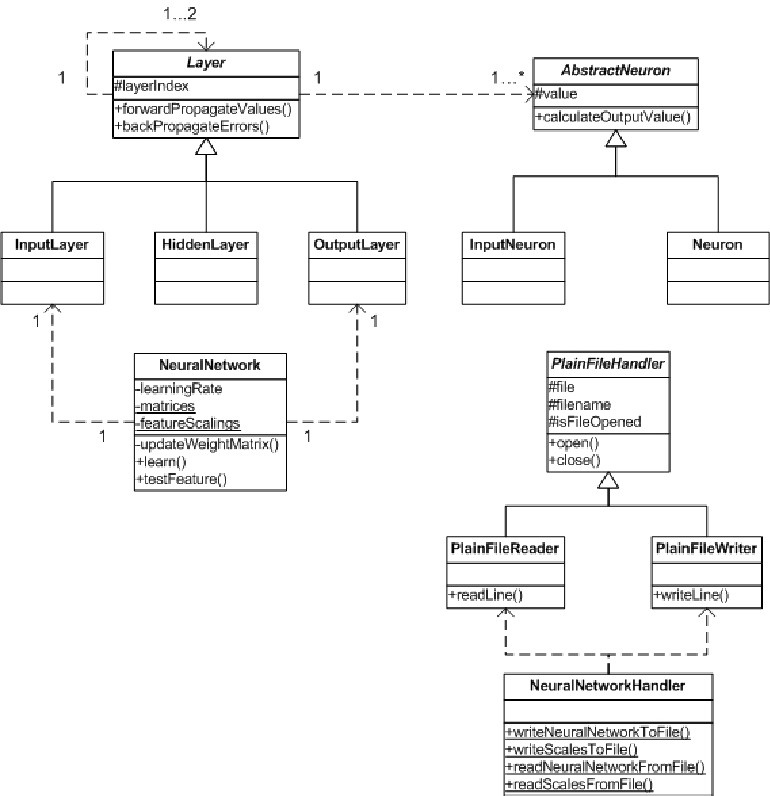
\includegraphics[width=1.0\columnwidth]{graphics/UML_WIDS}
	\end{center}
		
	\caption{The UML diagram of the neural network}
	\label{uml_wids}
\end{figure}

The abstract class {\em Abstractneuron} provides methods used by its subclasses labeled {\em InputNeuron} and {\em Neuron}. The only difference between these two classes is that the input neuron simply forwards the value received. The latter needs to be activated by calculating its output value by using the sigmoid function shown in section \ref{sec:activation}.

In addition to the neural network itself a helper class named {\em NeuralNetworkHandler} is provided which offers the possibility to read and write necessary values to and from plain text files. These values include the weights of all weight matrices in the network and the scaling values.

{\em {\bf Training the network}}

One single training cycle of the neural network works is shown in [xxx Appendix and Appendix]. It is important to note that training a neural network requires both, a forward and a backpropagation phase.

A {\em Trainer} class is responsible to start the training of a neural network. After the call of the {\em learn()} method the training starts. From now on all actions taken are the same for all layers:

As soon as all input values are set in the next layer its {\em forwardPropagateValue()} method is called which continues forward propagation. Next, the output value of each neuron in the current layer is calculated and given to the next layer as input values.

These steps described in the paragraph above are repeated for every single layer until the output layer is reached.

After finishing a forward propagation phase the errors of each neuron can be backpropagated.

The backpropagation phase starts at the output layer by calling the method {\em backpropagateErrors()}. Again, from now on the steps that are taken stay the same for all layers:

After calculating the error value of each single neuron in a specific layer this error is backpropagated until the first hidden layer. Note that the InputLayer is not affected by this calculation because the input layer itself is a pseudo layer which simply forwards the values coming from the outside.

Finally the weight matrix between each layer is updated by using the error values just calculated. That is the place where the learning happens.

{\em {\bf Testing the network}}

To test the neural network with a set of input values the only thing that needs to be done is to run through a forward propagation phase as described above. To receive the calculated output the method {\em getResultAt()} of the output layer is called.





























\chapter{Results}

\section{Introduction}

The following section explains the results obtained by the WIDS. First, the WIDS is tested [xxx] and shows the properties of the neural network that fit best for the WIDS.

\section{WIDS}

\subsection{Test environment}

The WIDS is trained and tested using different pcap files. The characteristics of these files are shown below in the table \ref{test_env}.

\begin{table}[htbp]
	\begin{center}
		\begin{tabular}{|l|l|l|p{60pt}|p{75pt}|}
		\hline
		&\bf{Train}&\bf{Test}&\bf{Association flood}&\bf{Disassociation flood} \\
		\hline
		Size&100 MB&100 MB&3 MB&2 MB\\
		\hline
		Time period&57 sec&-&-&-\\
		\hline
		Associations&5&-&200&0\\
		\hline
		Disassociations&4&-&-&-\\
		\hline
		Other packets&25412&20012&0&0\\
		\hline
		Rogue APs&no&yes&-&-\\
		\hline
		Unknown clients&no&yes&-&-\\
		\hline
		\end{tabular}
	\end{center}
	\caption{Test environment}
	\label{test_env}
\end{table}

{\em {\bf Packet distribution}}

Since the WIDS uses time relevant features to detect an attack it is important to know when something happens. The following graphs shows the packet distribution of the association and disassociation packets in the train and test file. The value in the y-axis show the packet count of the past two seconds.



\section{Preprocessor}

\section{Neural Network}

\begin{description}
%	\addtolength{\itemsep}{-1.5ex}

	\item [Initial weight values:] These values are especially important whenever a neural network is used which is trained by a small amount of training data or training cycles. Tests show [xxx see Appendix] that a neural network failed in learning a task because of too few training cycles
    \item [Number of hidden layers:] Tests show that an increasing number of hidden layers strongly raises the time needed to train the network but only slightly increases the quality of the resulting network
	\item [Number of neurons in the hidden layers:] Tests show that using too few neurons in a hidden layer can also result in a bad behaviour of the network
	\item [Learning rate:] It turned out that using a learning rate below the value 0.25 can reduce the performance of the neural network
	\item [Appearance of the sigmoid function:] [xxx nothing done so fasr]
\end{description}

\section{Choosing the learning rate}

\section{Choosing the number of neurons}

\section{Choosing the number of layers}

\chapter{Conclusion}

\section{Traditional Methods and Neural Networks}

\cite{nn_vs_traditional} states the question whether it is better or worse to use neural networks over traditional techniques to solve certain problems. The answer to that question is that this is "an unanswerable question" \cite[p.4]{nn_vs_traditional}. The problem lies in the way a neural network works.

First, the weight values that are given to an uninitialised network are chosen randomly. That means the obtained results differ even if the same training set is used.

Next, as described in section [xxx], the success to detect an intrusion attempt  highly depends on the features chosen for the input nodes. As a consequence the quality of the results using different features differ significantly.

Finally, the architecture of the network itself. Depending on the number of hidden layers and neurons used the performance of the network differs. As shown in section [xxx] the difference can be ...
